\documentclass[11pt,a4paper]{article}
\usepackage{amsmath}
\usepackage{url}


\usepackage{hyperref}

\newcommand{\RR}{\ensuremath{\rm I\!R}}
\newcommand{\NN}{\ensuremath{\rm I\!N}}
\def\n{{\hbox{\tiny{N}}}}
\def\t{{\hbox{\tiny{T}}}}

\usepackage{CMIS2018}
\usepackage{graphicx,subfig}
\usepackage[numbers,square,sort&compress]{natbib}
\bibliographystyle{unsrt}
\bibsep 0pt
\pagestyle{empty}

%% get rid of Large 'References' label
\renewcommand{\refname}{}
\newcommand{\inclps}[3]{\resizebox{#1}{#2}{\includegraphics{#3}}}

\graphicspath{{../figure/}}

\begin{document}
	
	\begin{center}
		
		% Title of the abstract
		{\Large\bf Formulations and extensive comparisons of 3D frictional contact solvers based on performance profiles}\vspace{11pt}
		
		% Full names of all authors
		{\large  \underline{Vincent Acary\textsuperscript
                    {1}}, Maurice Br\'emond and Olivier Huber}
		\vspace{11pt}
		
		% Affiliations and addresses
		{\small\itshape [1] INRIA \& LJK. Universit\'e Grenoble Alpes. France\\
                \protect{[2]} University of Wisconsin. Madison. USA}
	\end{center}
	
	%. Summary
	\begin{summary}
		\large
		This work reviews, details  and compares several numerical algorithms to solve 3D frictional contact problems. The comparisons is made with performance profiles comparing a dozen of methods and theirs variants over 2500 problems.
	\end{summary}
	\vspace{5pt}
        \vspace{-0.5cm}
\def\figillus{0.1\textheight}
\begin{figure}[htbp]
  \centering
  \subfloat[Cubes\_H8]{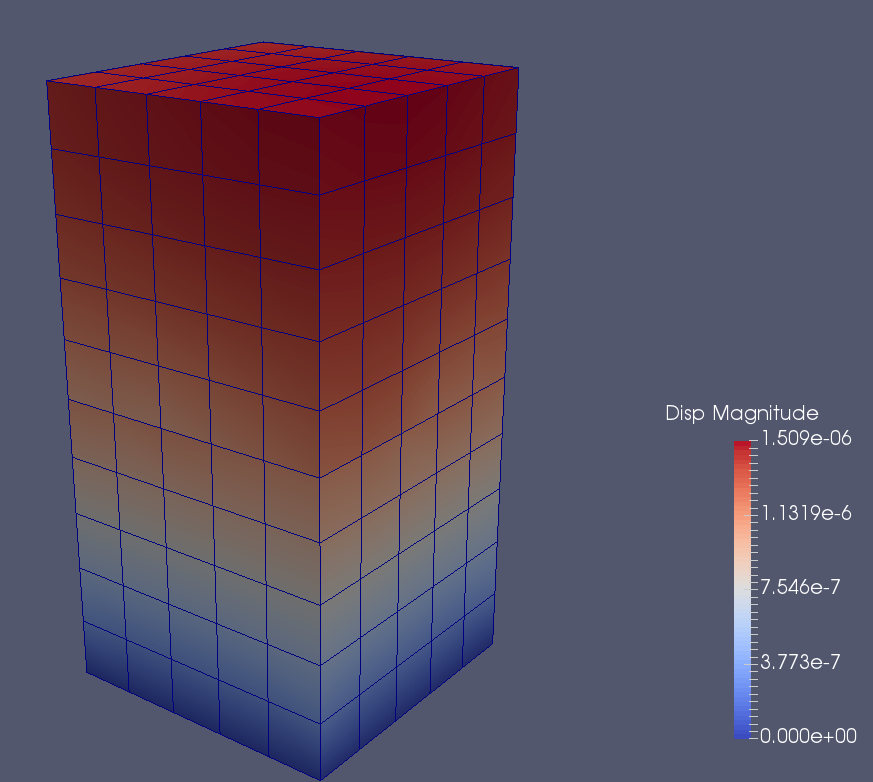
\includegraphics[height=\figillus]{figure/Cubes_H8_5.png}}
  \subfloat[LowWall\_FEM]{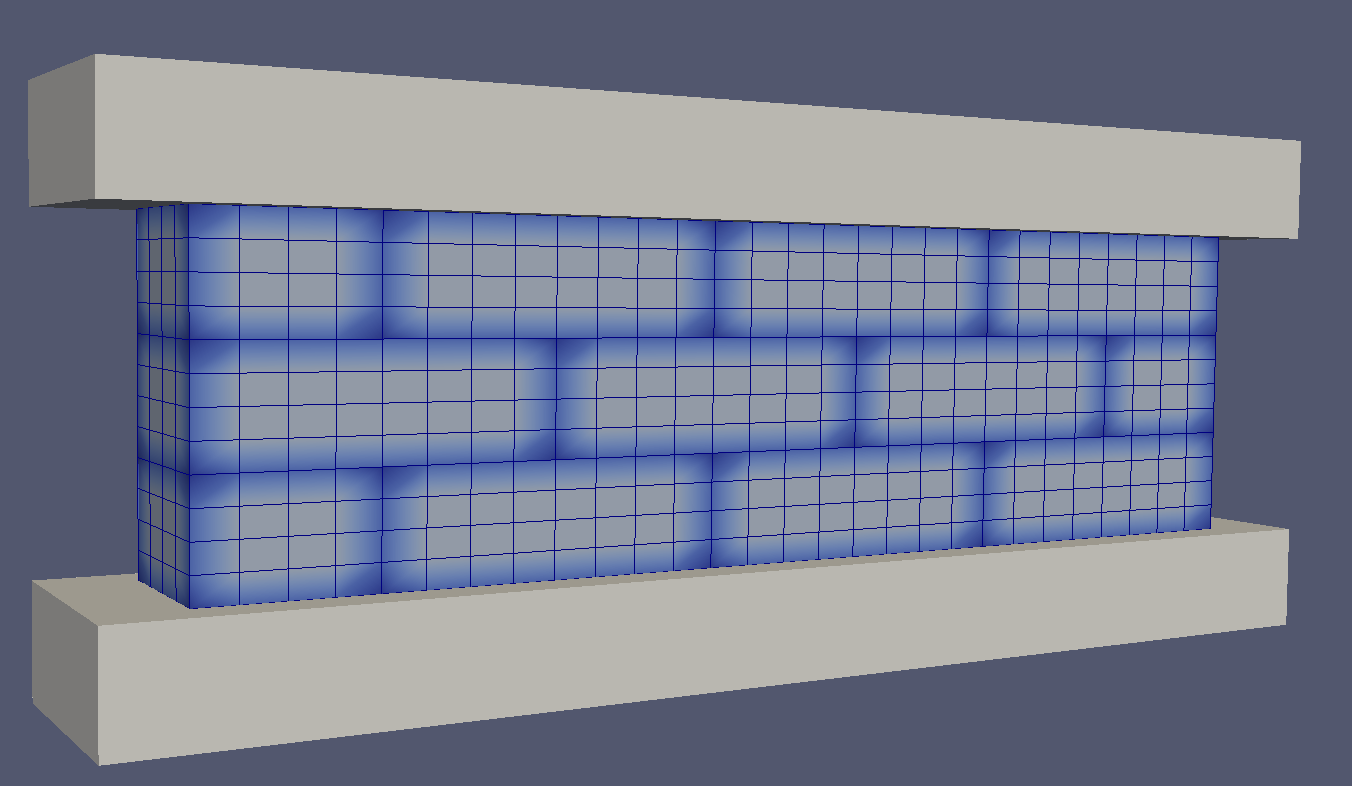
\includegraphics[height=\figillus]{figure/LowWall_FEM.png}}
  \subfloat[Aqueduct\_PR]{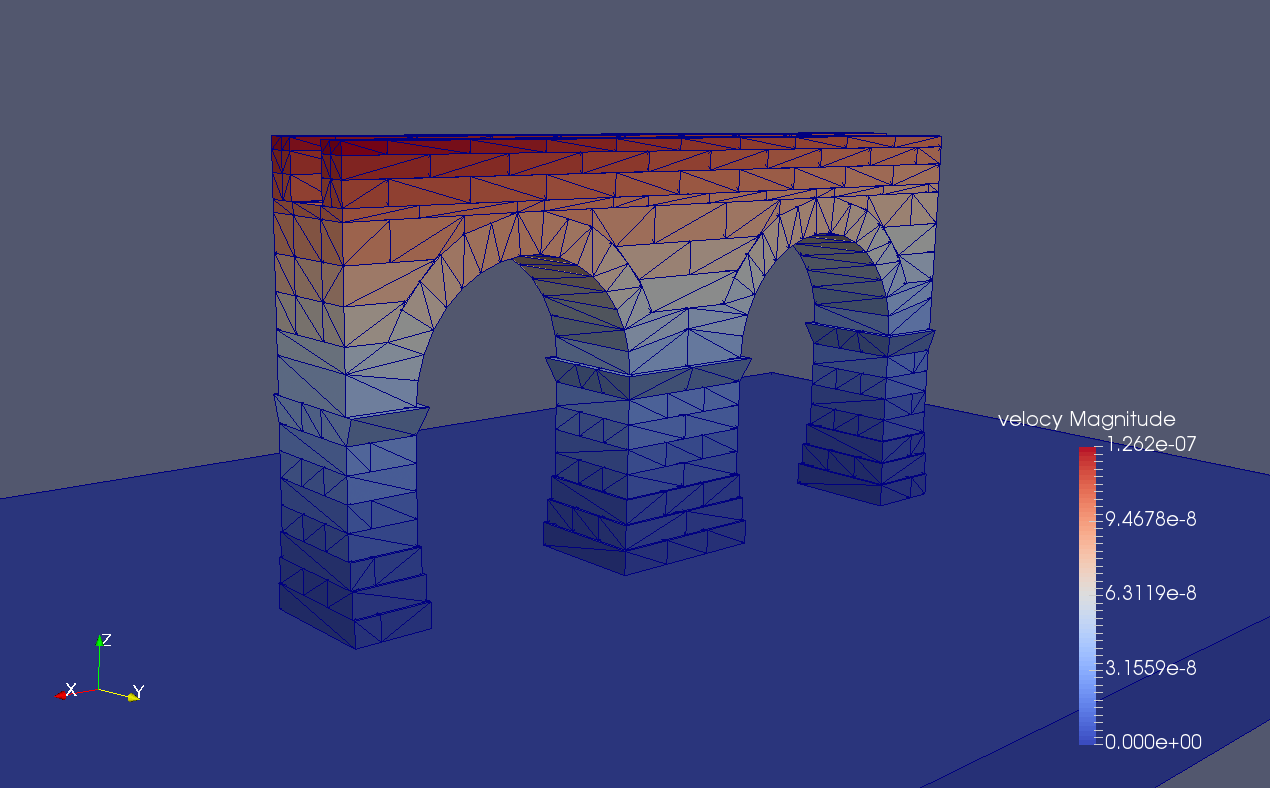
\includegraphics[height=\figillus]{figure/Aqueduc_PR.png}}
  %\subfloat[Bridge\_PR]{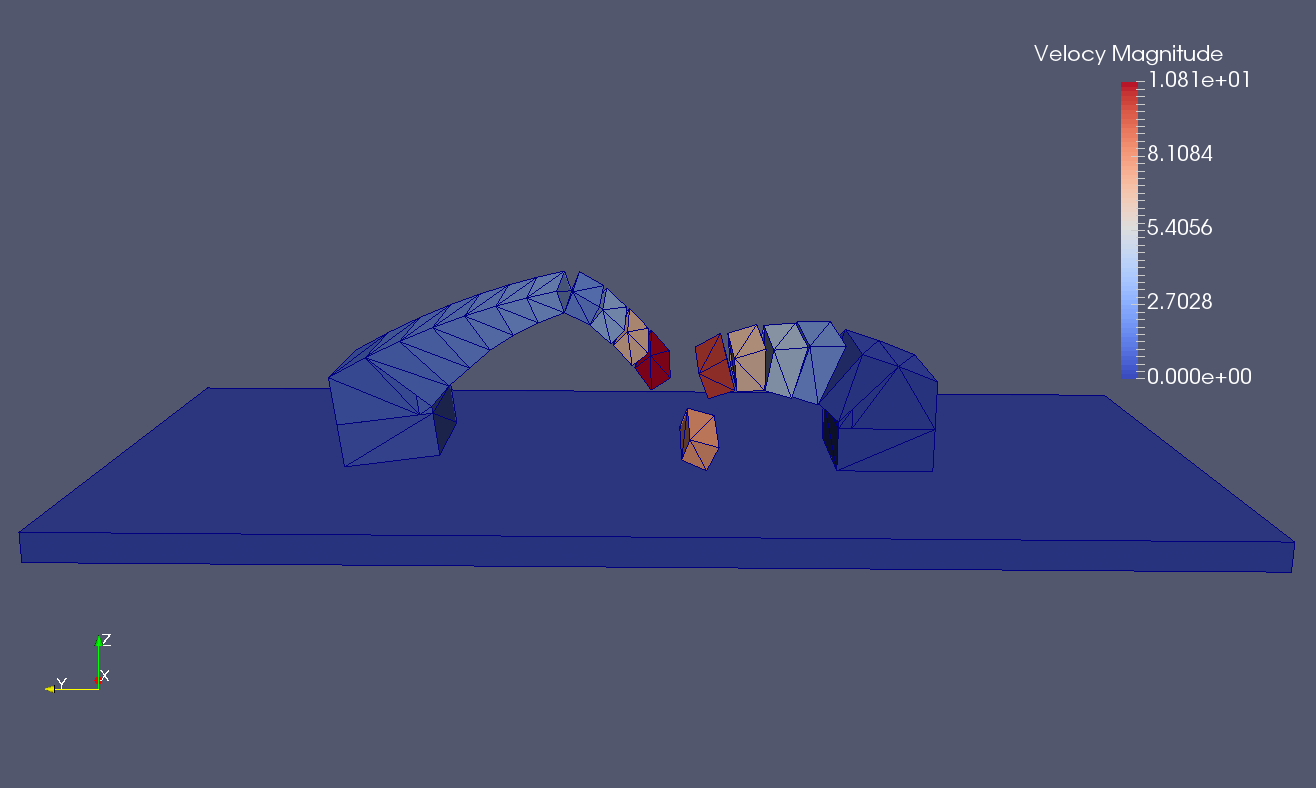
\includegraphics[height=\figillus]{figure/Bridge_PR_1.png}}
  %\subfloat[100\_PR\_Periobox]{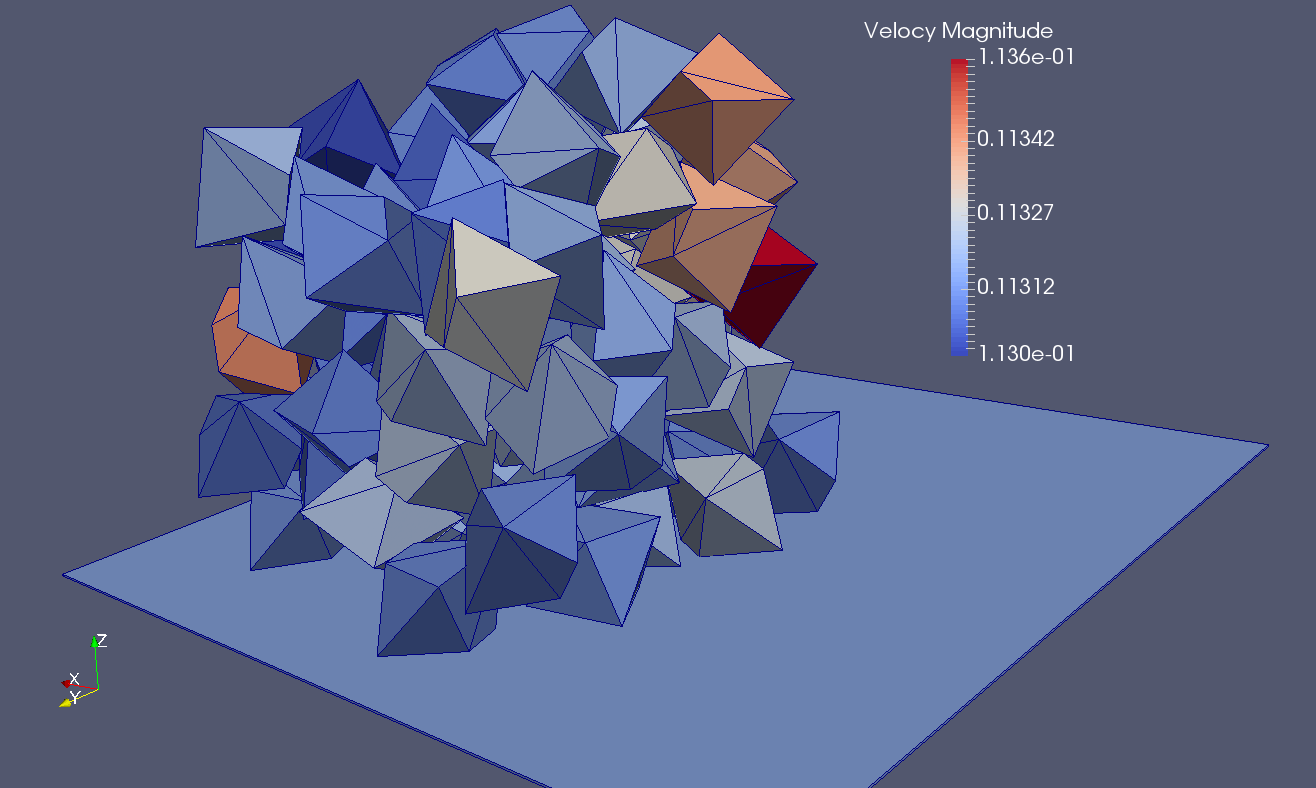
\includegraphics[height=\figillus]{figure/100_PR_PerioBox.png}}
  %\subfloat[945\_SP\_Box\_PL]{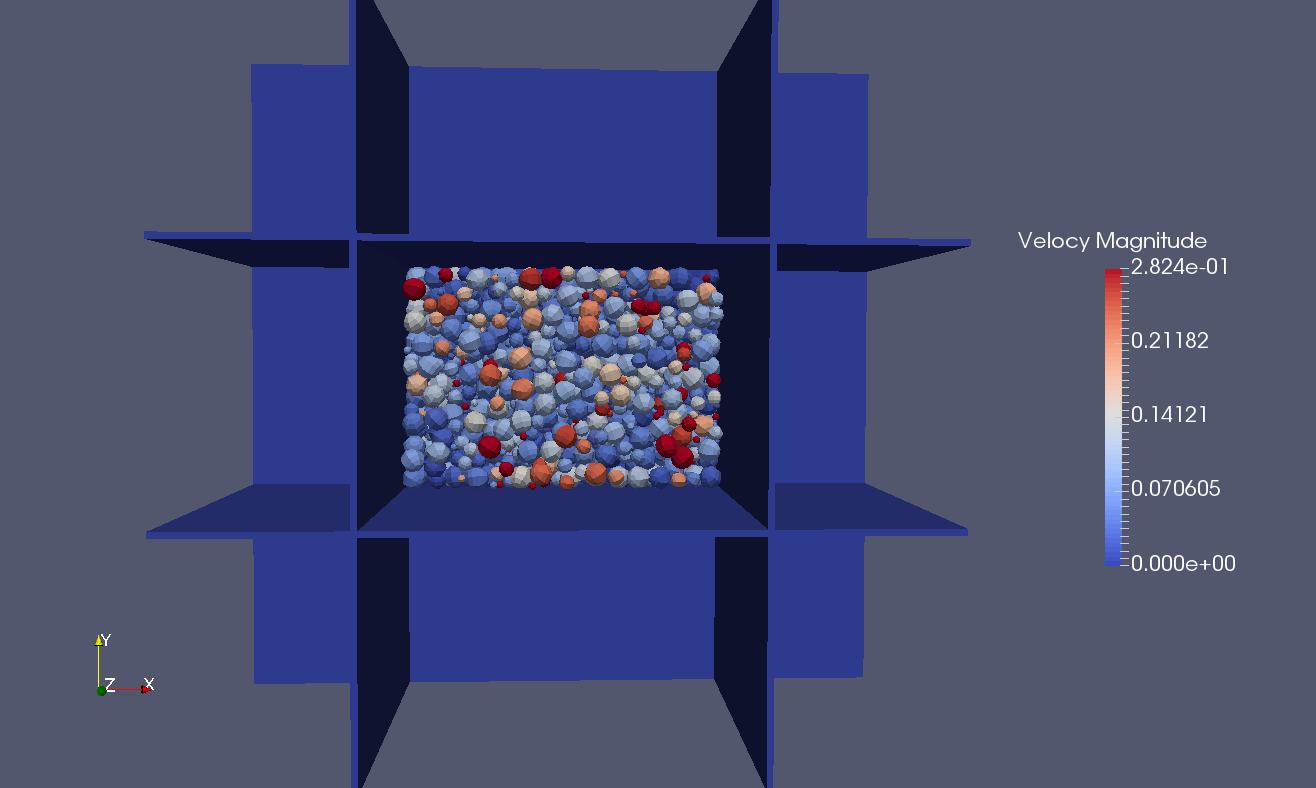
\includegraphics[height=\figillus]{figure/945_SP_Box_PL.png}}
  % \subfloat[Capsules]{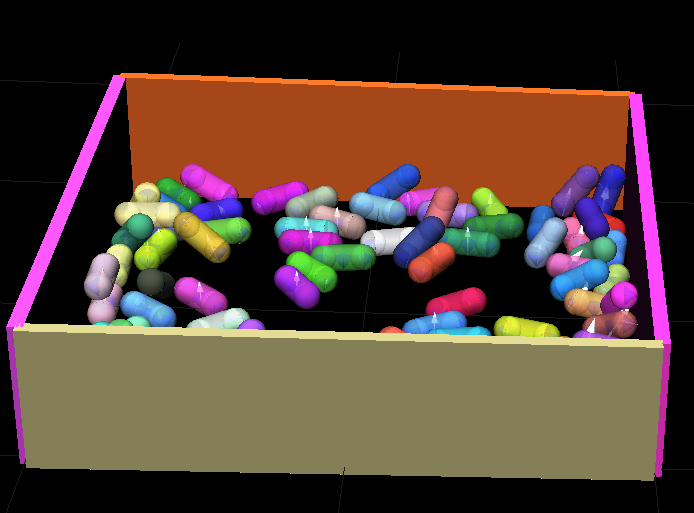
\includegraphics[height=\figillus]{figure/Capsules.png}$\quad$}
  %\subfloat[Chain]{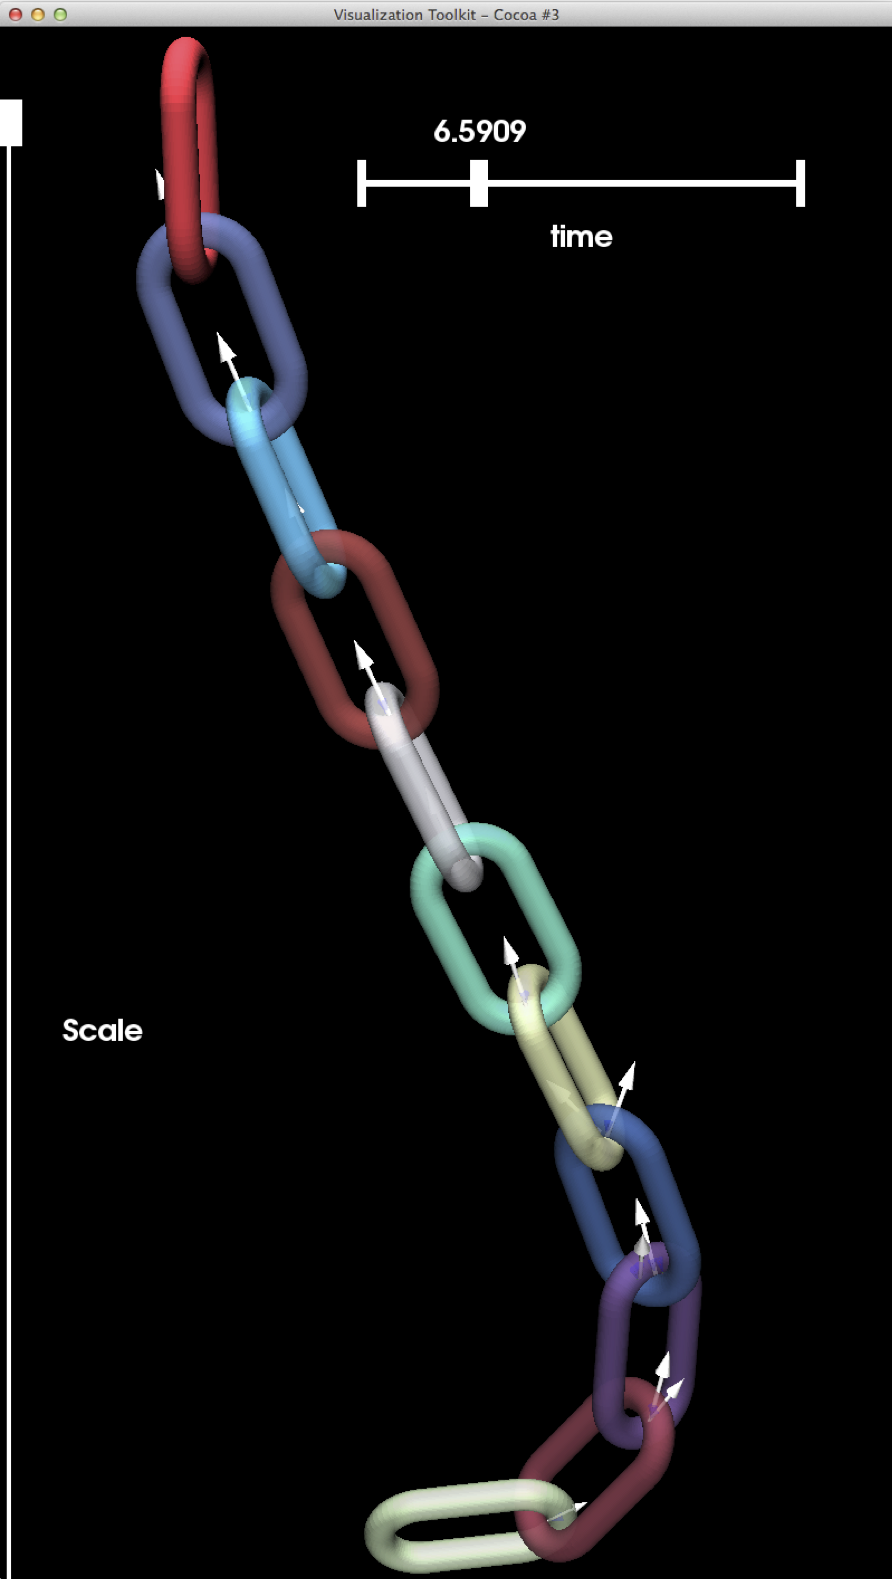
\includegraphics[height=\figillus]{figure/Chains.png}$\quad$}
  %\subfloat[KaplasTower]{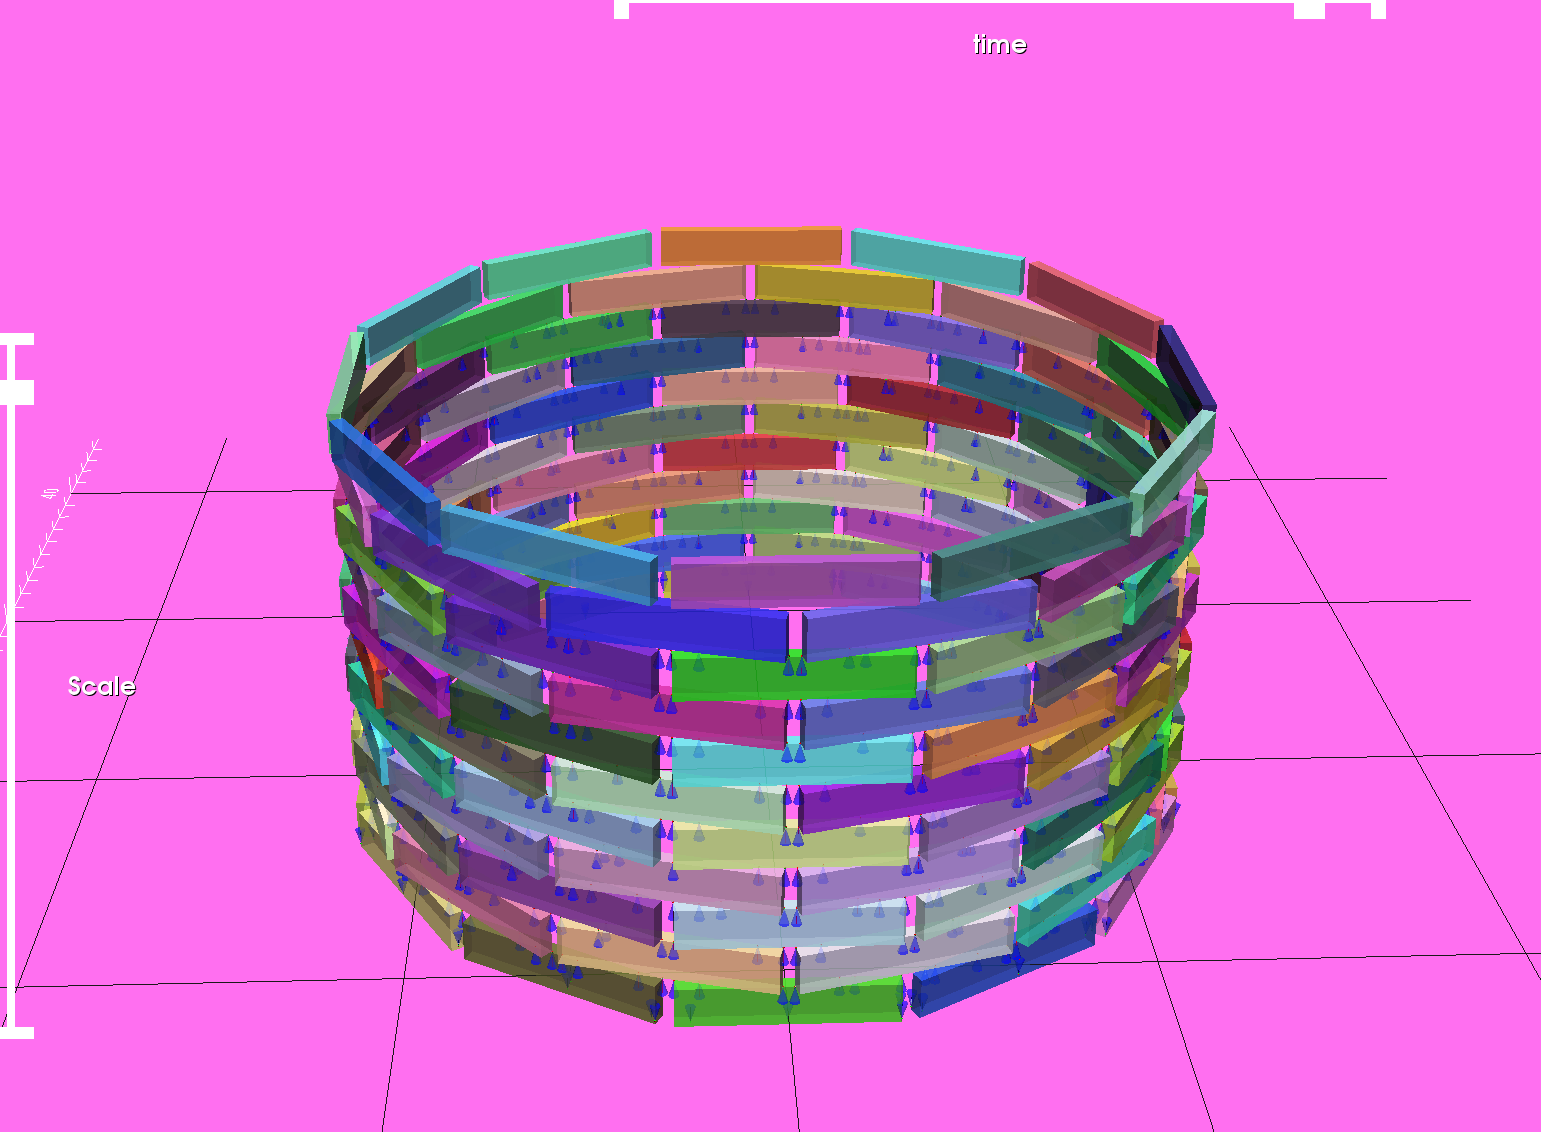
\includegraphics[height=\figillus]{figure/KaplasTower.png}$\quad$} \subfloat[BoxesStack]{$\quad$$\quad$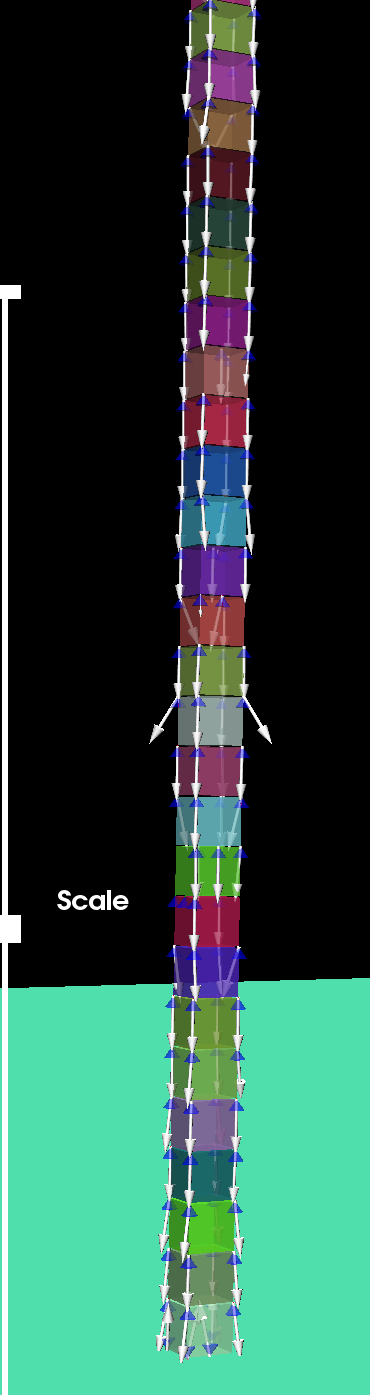
\includegraphics[height=\figillus]{figure/BoxesStack.png}$\quad$$\quad$}\\
\subfloat[Chute\_4000]{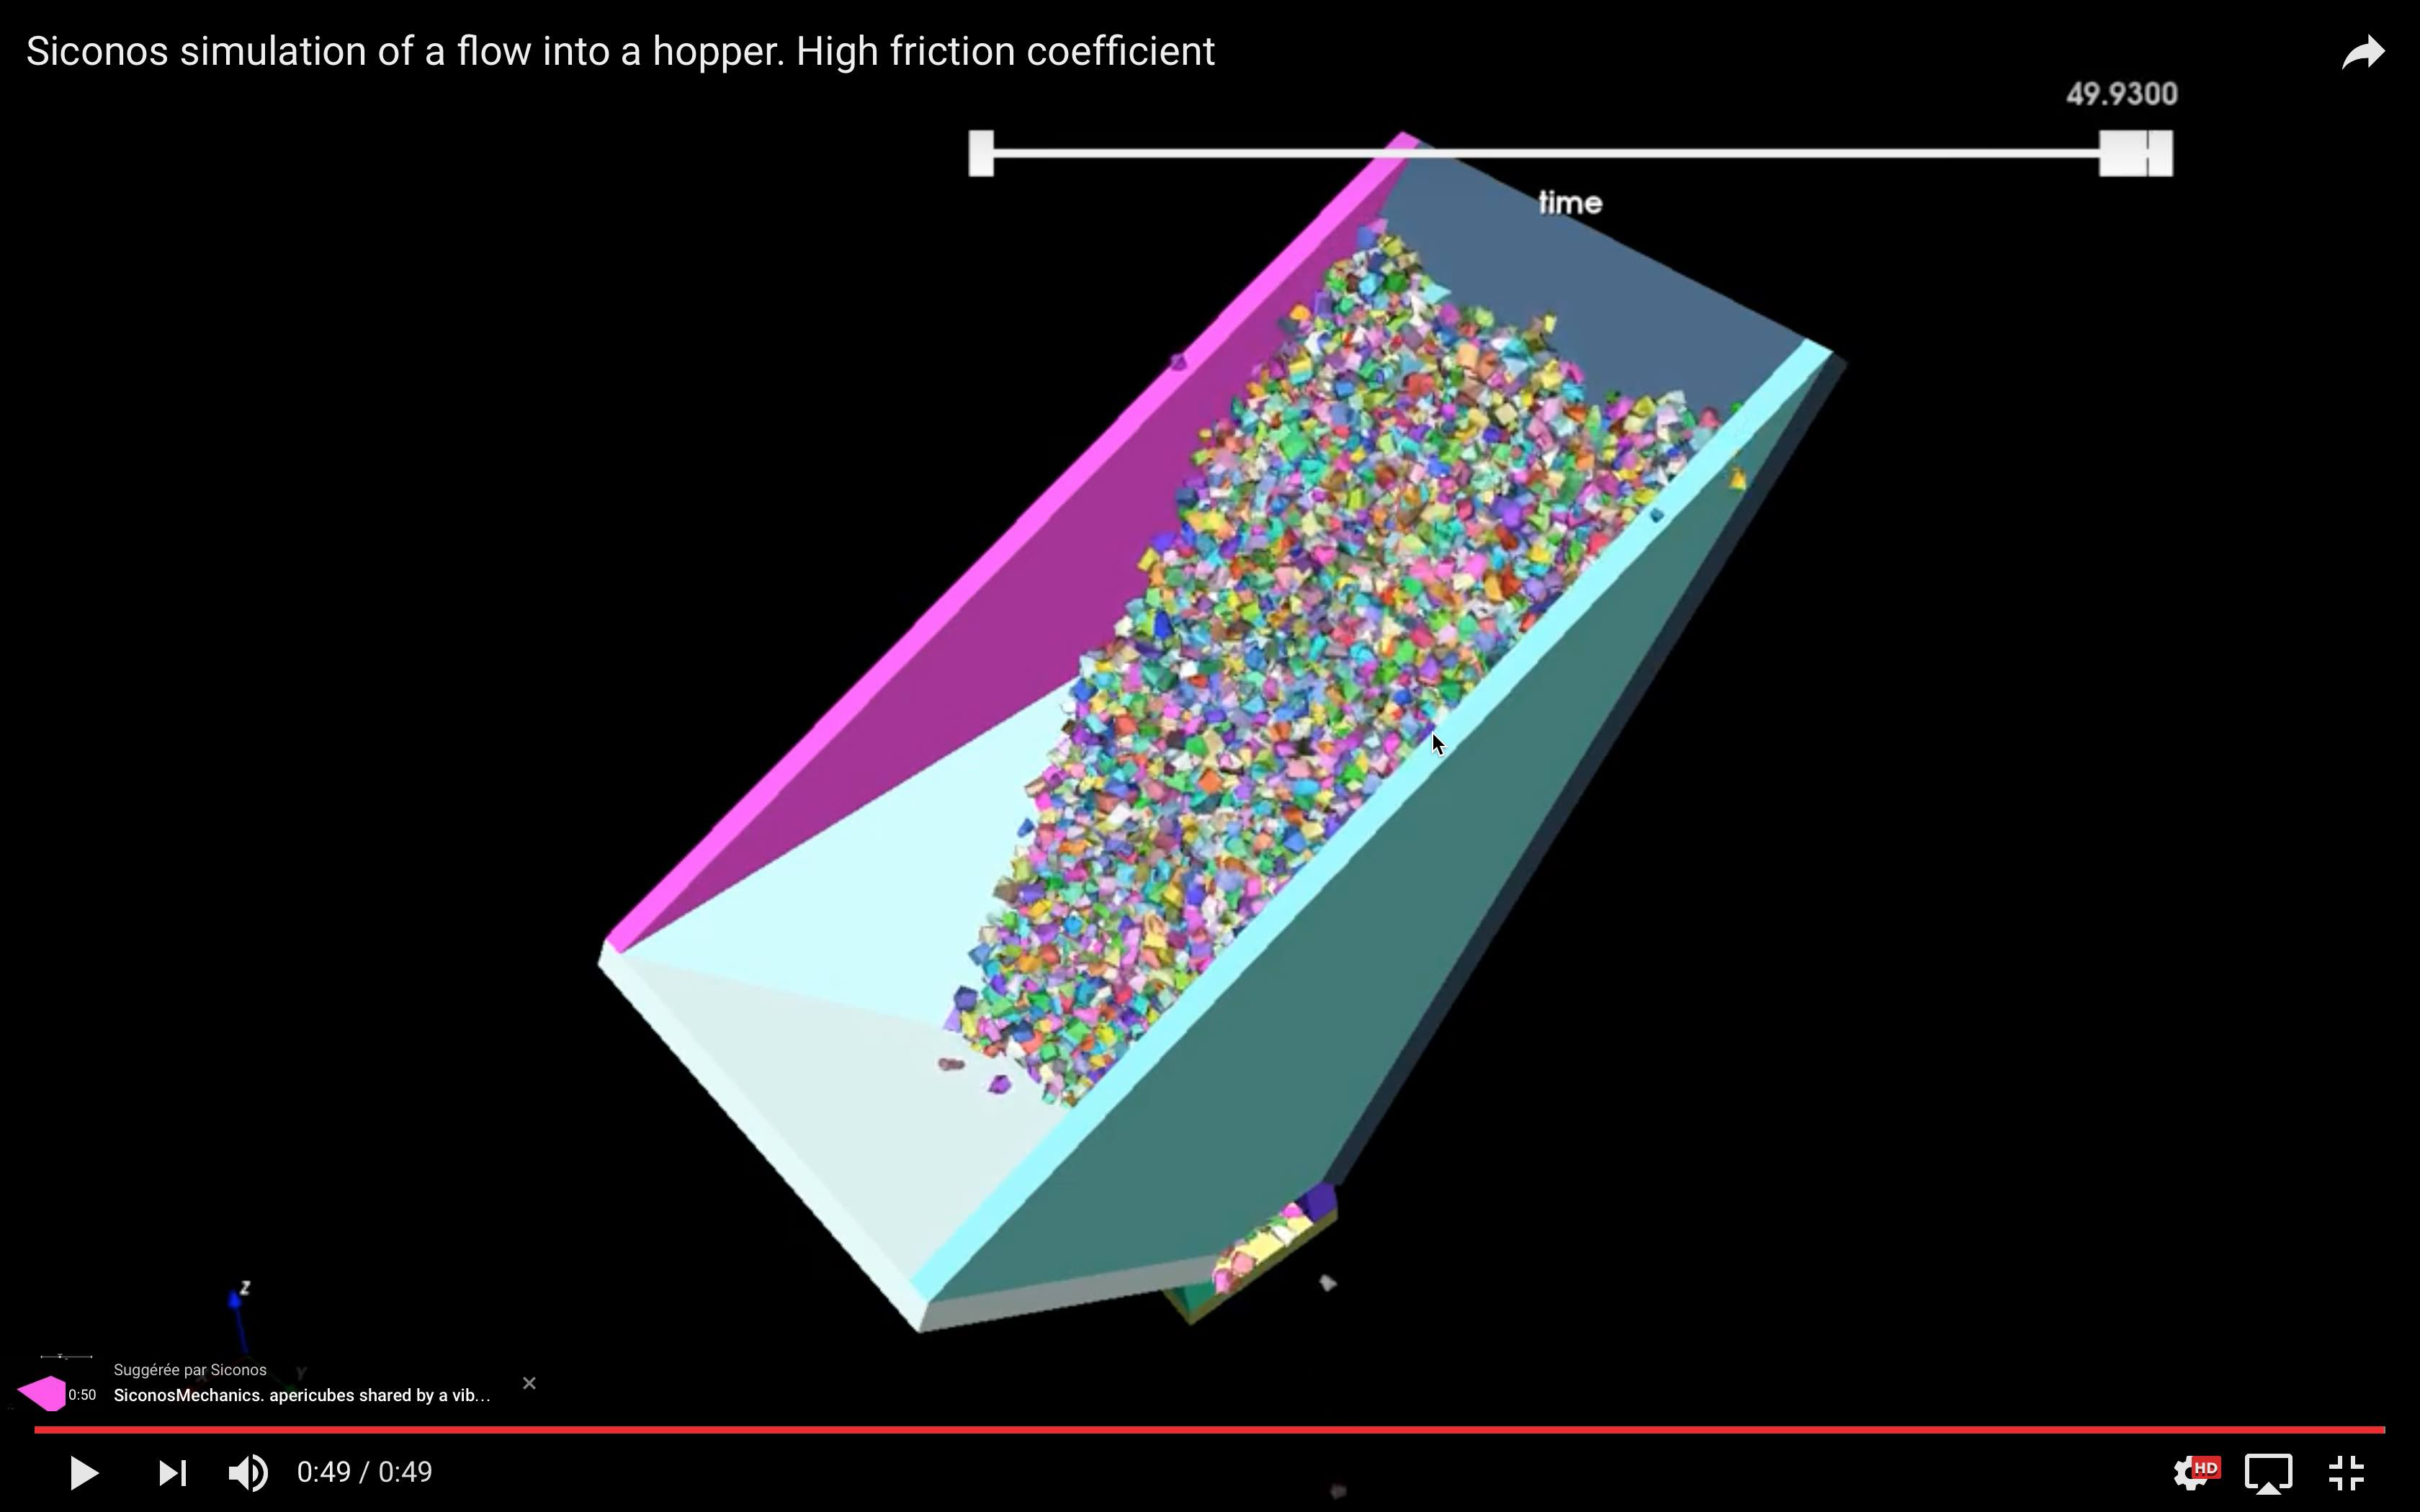
\includegraphics[height=\figillus]{figure/Chute_1000_light.jpg}$\quad$$\quad$$\quad$$\quad$}
  \caption{Illustrations of the FClib test problems}
  \label{fig:fclib}
\end{figure}
\vspace{-1cm}\section{Introduction}

In this talk, we want to discuss possible numerical solution procedures for the following discrete frictional contact problem~\cite{Acary.Brogliato2008}.   Let $n_c\in \NN$ be the number of contact points and $n\in\NN$ the number of degree of freedom. Given a symmetric positive (semi-)definite matrix ${M} \in \RR^{n \times n}$, a vector $ {f} \in \RR^n$, a matrix  ${H} \in \RR^{n \times m}$ with $m= 3n_c$, a vector $w \in \RR^{m}$ and a vector of coefficients of friction $\mu \in \RR^{n_c}$, find three vectors $ {v} \in \RR^n$, $u\in\RR^m$ and $r\in \RR^m$ such that
\begin{equation}\label{eq:soccp1}
  \begin{array}{rcl}
    M v = {H} {r} + {f}, &
    u = H^\top v + w,  &
    \hat u = u + g(u), \quad 
                         K^\star \ni {\hat u} \perp r \in K,
  \end{array}
\end{equation}
where $g(u)$ is a nonsmooth function and $K\subset \RR^{3 n_c}$ is a Cartesian product of second order cone in $\RR^3$.   For each contact $\alpha$, the unknown variables  $u^\alpha\in\RR^3$ (velocity or gap at the contact point) and $r^\alpha\in\RR^3$ (reaction or impulse) are decomposed  in a contact local frame $(O^\alpha,{\sf N}^\alpha,{\sf T}^\alpha)$ such that $u^\alpha = u^\alpha_{\n} {\sf N}^\alpha +   u^{\alpha}_{\t}, u^\alpha_{\n} \in \RR, u^\alpha_{\t} \in \RR^2$ and  $r^\alpha = r^\alpha_{\n} {\sf N}^\alpha +   r^{\alpha}_{\t}, r^\alpha_{\n} \in \RR, r^\alpha_{\t} \in \RR^2$.
% The Coulomb friction cone for a  contact $\alpha$ is defined by $K^{\alpha}  = \{r^\alpha, \|r^\alpha_\t \| \leq \mu^\alpha |r^\alpha_\n| \}$ and the set $K^{\alpha,\star}$ is its dual.  
The set $K$ is the cartesian product of Coulomb's friction cone at each contact, that is
\begin{equation}
  \label{eq:CC}
  K = \prod_{\alpha=1\ldots n_c} K^{\alpha}  = \prod_{\alpha=1\ldots n_c} \{r^\alpha, \|r^\alpha_\t \| \leq \mu^\alpha |r^\alpha_\n| \}
\end{equation}
and $K^\star$ is dual.
The function $g$ is defined as $g(u) = [[\mu^\alpha  \|u^\alpha_\t\| {\sf N}^\alpha]^\top, \alpha = 1\ldots n_c]^\top$.

\vspace{-0.5cm}\section{Origin of the problem}
  This problem is at the heart of the simulation of mechanical systems with 3D Coulomb's friction and unilateral constraints. It might be the result of the time--discretization by event--capturing time--stepping methods or event--detecting (event--driven) techniques of dynamical systems with friction or the result of a space--discretization (by FEM for instance) of the quasi-static problems of frictional contact mechanics~\cite{Acary.Cadoux2013}. On the mathematical programming point of view, the problem appears as Second Order Cone Complementarity Problem (SOCCP). If the nonlinear part of the problem is neglected ($g(u)=0$), the problem is an associated friction problem with dilatation, and by the way, is a gentle Second Order Cone Linear Complementarity Problem (SOCLCP) with a positive matrix $H^\top M^{-1} H$ (possibly semi--definite). When the non-associated character of the friction is taken into account through $g(u)$, the problem is non monotone and nonsmooth, and then very hard to solve efficiently.

\vspace{-0.6cm}\section{Formulations based on numerical optimization}
  
In this talk we will recall a result for the problem ~(\ref{eq:soccp1}) which ensures that a solution exists~\cite{Acary.ea_ZAMM2011}. Then, we will list several algorithms that have been previously developed for solving the SOCCP~(\ref{eq:soccp1}):
\begin{itemize}
  \setlength\itemsep{0em}
\item Variational inequalities solvers: fixed point with projection and extragradients techniques with self-adapting step rule.
\item Nonsmooth equations solvers: semi--smooth and generalized Newton methods with line-searches
\item Block--splitting (Gauss-Seidel Like) and projected suroverrelaxation (PSOR).
\item Proximal point algorithms
\item Optimization based solvers: Panagatiopolous approach, Czech school approach (Tresca successive approximations) and convex SOCQP relaxation.
\end{itemize}
\vspace{-0.6cm}\section{Extensive comparisons}
The goal of this work is to compare on a large set of problems the methods that we found in the literature. To this end, we develop an open collection of discrete frictional contact problems called FCLIB\footnote{\href{https://frictionalcontactlibrary.github.io/index.html}{https://frictionalcontactlibrary.github.io/index.html}} in order to offer a large library of problems to compare algorithms on a fair basis.  In this work, this collection is solved with the software {\sc Siconos} and its component {\sc Siconos/Numerics}\footnote{\href{http://siconos.gforge.inria.fr}{http://siconos.gforge.inria.fr}} .


\vspace{-0.5cm}\section{Conclusions}

On one hand, we will show that algorithms based on Newton methods for nonsmooth equations solve quickly the problem when they succeed, but suffer from robustness issues mainly if the matrix $H$ has not full rank. On the other hand, the 
iterative methods dedicated to solving variational inequalities are quite robust but with an extremely slow rate of convergence. To sum up, as far as we know there is no option that combines time efficiency and robustness. This presentation will be a summary of the work detailed in the following technical report~\cite{acary:hal-01630836}

\vspace{-0.3cm}\subsection{References}
\vspace{-0.5cm}\setlength{\bibsep}{0.5em}
\small
\bibliographystyle{plain}
\bibliography{biblio}


% \begin{thebibliography}{9} \vspace{-1em}
% 	\bibitem[1]{Wriggers06} P.~Wriggers. \newblock \emph{Computational Contact Mechanics}, \newblock 2nd ed., Springer, 2006.
% 	\bibitem[2]{ZavariseWriggers00} G.~Zavarise and P.~Wriggers, \newblock
% 	Contact with friction between beams in 3-D Space, \newblock \emph{Int. J. Num. Meth. Engng.}, 49:977-1006, 2000.
% 	\bibitem[3]{LaursenSimo93} T.~Laursen and J.C.~Simo, \newblock A continuum-based finite element formulation for the implicit solution of multibody, large deformation
% 	frictional contact problems, \newblock \emph{Int. J. Num. Meth. Engng.}, 36:3451--3485, 1993.
% \end{thebibliography}
	
\end{document}






%%% Local Variables:
%%% mode: latex
%%% TeX-master: t
%%% End:
